% Chapter 2

% variables
\newcommand{\pdirtwo}{chapters/chapter2/plots}

\chapter{The NA64 experiment} % Main chapter title

\label{chapter2} % For referencing the chapter elsewhere, use \ref{Chapter2} 

% ----------------------------------------------------------------------------------------

\section{Experimental Technique}
\label{chapter2:sec:experimental-technique}

\subsection{invisible decay mode}
\label{chapter2:sec:experimental-technique-invis}

\subsection{visible decay mode}
\label{chapter2:sec:experimental-technique-vis}

\section{Experimental setup}
\label{chapter2:sec:experimental-setup}

\subsection{The invisible mode setup}
\label{chapter2:sec:invismode}

\subsection{The visible mode setup}
\label{chapter2:sec:vismode}

The method of the search for $\aee$ (or $\xdecay$) decays is detailed in \cite{Gninenko:2013rka, Andreas:2013lya, gkkk1, DMsimulation}. Here, we review it briefly. The $\DM$ is produced via scattering of 150 GeV electrons off nuclei of an active target-dump. The $\DM$ production is followed by its decay into $\ee$ pairs:
\begin{equation}
e^- + Z \to e^- + Z + \DM   ;~ \DM\to \ee \,.
\label{ea}
\end{equation}


\begin{figure}[tb]
\centering
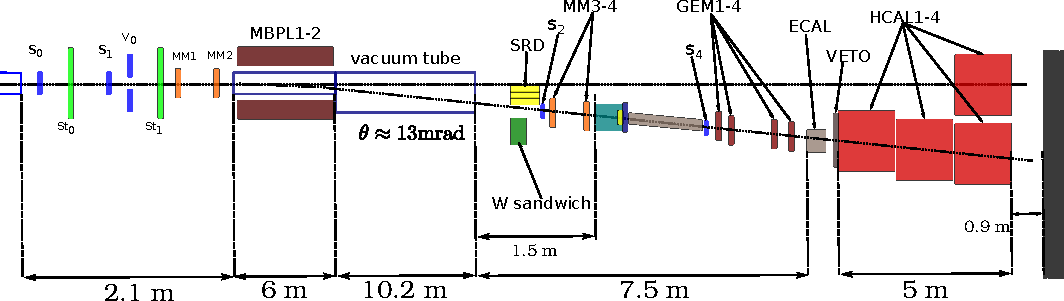
\includegraphics[width=1.\textwidth]{\pdirtwo/NA64_setup_2018_visible.pdf}
\caption[NA64 visible mode setup 2018]{The setup to search for $\DM$$\to \ee$  decays of the bremsstrahlung $\DM$ produced in the reaction
$eZ \to eZ+\DM $ of the 150 GeV electrons incident on the active WCAL target.}
\label{fig:setup-2018}
\end{figure}

The NA64 experiment searched for these decays using the H4 beam line of the CERN Super Proton Synchrotron (SPS) delivering about  $\simeq 5\times 10^6~e^-$ every 4.8 seconds. The setup used for this search is shown in Fig.\ref{fig:setup-2018}. A spectrometer made of a bending magnet combined with trackers measures the particle momentum. The magnet allows as well a very efficient electron identification (ID) using a Synchrotron Radiation Detector(SRD). Hadrons are additionally suppressed using a high efficiency VETO and a set of 3 hadronic calorimeter modules (HCAL) placed at the end of the setup. To measure the energy of the $\ee$ in signal events a highly-segmented electromagnetic-calorimeter (ECAL) is placed downstream of the decay volume. The signal region is defined by the sum of energy deposited in both calorimeters being compatible to the original beam energy. Additionally, the energy deposited in the last layer of the WCAL (W$_2$) is required to be lower than one Minimum Ionizing Particle (MIP) to suppress punch-through from the electromagnetic shower.

The allowed coupling $\epsilon$ for the $\DM$ can be as high as $1.4 \times 10^{-3}$, resulting in a very short decay length of few mm. Therefore, to boost the signal yield one should reduce the length of the active target to enhance the number of decays outside the dump. Additionally, for an unambiguous signature of the $\DM$ production it is crucial to reconstruct the invariant mass of the particle's decay. The small decay angle of $\DM$ ($\sim$0.3 mrad) makes this task particularly challenging. Therefore, a long decay volume must be used to resolve the two tracks.

\section{Detectors}
\label{chapter2:sec:detectors}

\subsection{The Trigger system}
\label{chapter2:sec:detectors-trigger}

\subsection{The Electromagnetic Calorimeter (ECAL)}
\label{chapter2:sec:detectors-ecal}

\subsection{The Hadronic Calorimeter (HCAL)}
\label{chapter2:sec:detectors-hcal}

\subsection{The Synchrotron radiation detector (SRD)}
\label{chapter2:sec:detectors-srd}

\subsection{The Veto system}
\label{chapter2:sec:detectors-veto}

\subsection{The Tracking system}
\label{chapter2:sec:detectors-tracking}

\subsection{The data Acquisition system (DAQ)}
\label{chapter2:sec:daq}

%%% Local Variables:
%%% mode: latex
%%% TeX-master: t
%%% End:
